If we look at the graph of $\chi'$ for a threee level system we can see that we will get a region of very steep positive dispersion.
\begin{figure*}[h!]
	\centering
	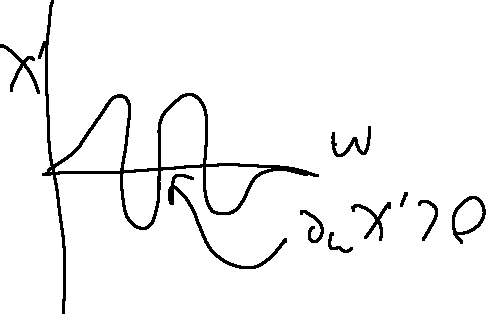
\includegraphics[width=10cm]{images/11-26-1.png}
	\caption*{Plot of 3LS $\chi'$}
\end{figure*}
Using this formula, when the slope becomes very high we will have light that has a group velocity much much slower than normal (as slow as 10m/s).
How do we understand this? We can think of this as the adiabatic passage of a dark state. If we start in the dark state, and send in a probe pulse then we will see our population remain in the dark state *which begins as $\ket{1}$.
\begin{figure*}[h!]
	\centering
	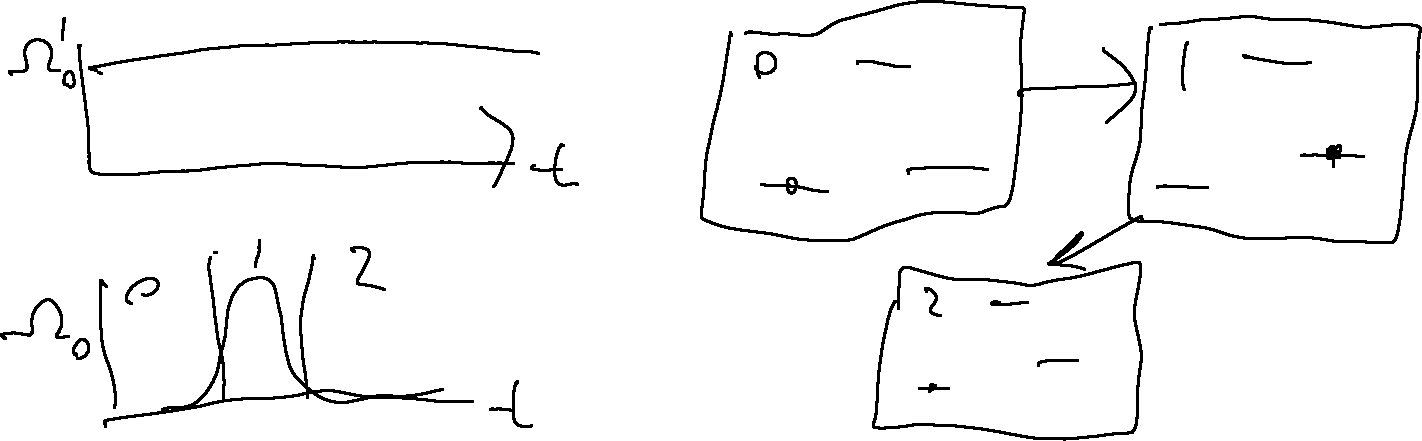
\includegraphics[width=10cm]{images/11-26-2.png} \\
	\caption*{Plot of the state as a pulsed probe is incident on the sample}
\end{figure*}
Once the probe arrives we see the population move to three, and then back to one as the pulse leaves.

Looking at the field we see this as an energy exchange. First we put energy from the field into the state for the transition from $\ket{1}\to\ket{3}$. Then we take energy out of the state and put it back into the field going from $\ket{3}\to\ket{1}$.
The rate of energy exchange is $~\Omega_0'$, so our group velocity scales with $\Omega_0'$. It can be shown that $v_g\propto\Omega_0'\ ^2$. This can be used to store light. If $\alpha L \gg 1$ then the probe is completely absorbed by the medium.
After this our $\rho_{13}$ is not zero. Not only not this value contains the information of the probe pulse. Therefore we say the probe pulse is stored in the medium as the coherence.

We want to know how to retrieve this information. In order to do this we simply need to apply a pump field to our sample.
\begin{figure*}[h!]
	\centering
	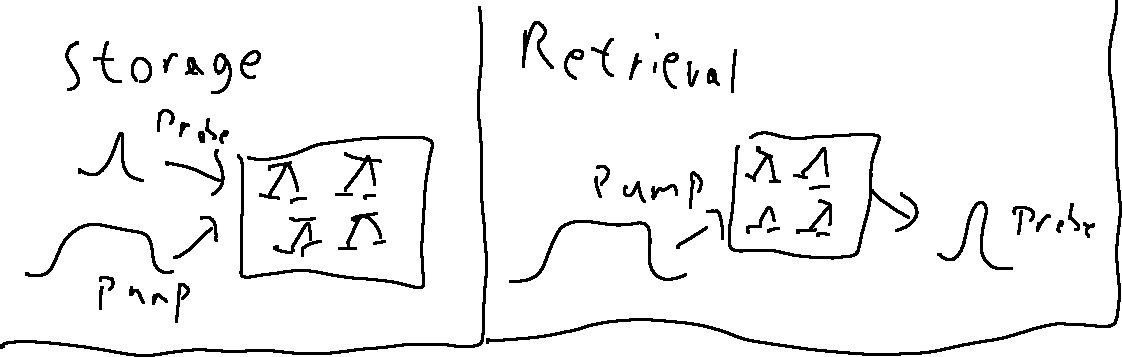
\includegraphics[width=10cm]{images/11-26-3.png}
	\caption*{Storage and retrieval of an optical field}
\end{figure*}
\subsection{Summary}
We introduced the idea of dark states, and used this idea to introduce the phenomena of coherent population trapping (related to $\rho_{22}$) and electromagnetically induced transparency (related to $\chi$).
Using adiabatic passage we also could see STIRAP, slow light and light storage. In all these our nonradiative coherence $\rho_{13}$ plays a central role.

Additionally we can see that for other types of three level systems (V or cascade). In both of these systems our $\rho_{13}$ decays via spontaneous emission, so it is shorter lived and these techniques aren't as powerful.
Finally we can look at EIT as a result of classical coupled harmonic oscilators.
\section{Mechanical effects of light}
\subsection{Overview}
The key insight of this section will be that light carries momentum (you can see this in Maxwell's equations).
In quantum mechanics we know that the momentum of a photon is $\hbar\bm{k}$. Therefore optical interactions must satisfy momentum conservation. The force applied is typcially quite small in macroscopic scales (~1W lasers will apply ~1nN of force).
Looking at the interaction of an atom with a photon instead, we see that not only will the atom's state change, but so will it's momentum, i.e. the change will be $\Delta\bm{p} = \hbar\bm{k}$, similarly for emission $\Delta\bm{p} = -\hbar\bm{k}$,
where in both of these $\bm{k}$ is the photon's wave vector.
\begin{figure*}[h!]
	\centering
	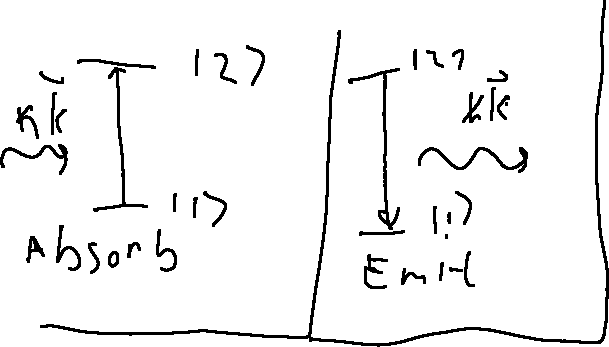
\includegraphics[width=10cm]{images/11-26-4.png}
	\caption*{Change in momentum from Emision and Absorption}
\end{figure*}
\subsection{Radiation Pressure}
This is sometimes called dissipative force. 

We start by ignoring spontatneous emission. This process will be absorption followed by stimulated emission, and since the wave vector will be the same for the absorbed and emitted light, then the overall change in momentum is zero.

\begin{figure*}[h!]
	\centering
	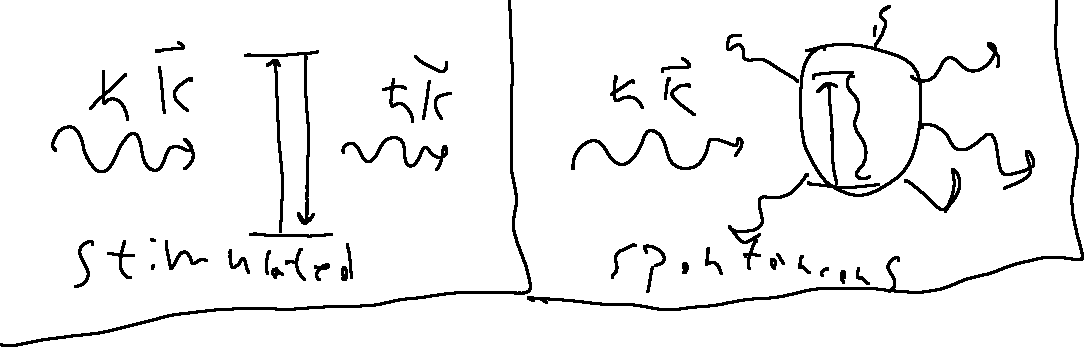
\includegraphics[width=10cm]{images/11-26-5.png}
	\caption*{Change in momentum from Stimulated and Spontaneous emission}
\end{figure*}

If we instead include the stimulated emission process, then we have $\hbar\bm{k}$ absorbed, and the $\hbar\bm{k}'$ emitted, where $\bm{k}'$ is the same magnitude as $\bm{k}$ but points in a random direction. On average the momentum change from the emission is zero,
therefore the total momentum change is going to be $\hbar\bm{k}$. If we continously shine a laser on a sample that will spontaneously emit photons, then the total change will be $\hbar\bm{k}\gamma_2\rho_{22}\Delta t$.
Therefore the force will be:
\begin{align*}
	\bm{F} &= \frac{\expval{\Delta \bm{p}}}{\Delta t} \\
	\bm{F} &= \hbar\bm{k}\gamma_2\rho_{22} \\
	\bm{F} &= \hbar\bm{k}\gamma_2\frac{\Omega_0|^2\gamma}{2\gamma_2}\frac{1}{\delta^2 + \gamma^2}
\end{align*}
And clearly the maximum force must be (because in steady state $\rho_{22} \leq \frac{1}{2}$):
\begin{align*}
	\bm{F}_\text{max} &= \frac{1}{2}\hbar\bm{k}\gamma_2
\end{align*}
\subsection{Doppler cooling}
We start by briefly reviewing the Doppler shift. If we look at an atom moving with a velocity $v$, we can say energy and momentum conservation together yield:
\begin{align*}
	m\bm{v} + \hbar\bm{k} &= m\bm{v}' \\
	\frac{1}{2}mv^2 + \hbar\omega_1 + \hbar \omega &= \hbar\omega_2 + \frac{1}{2}mv'\ ^2 \\
	\frac{1}{2}mv^2 + \hbar\omega_1 + \hbar \omega &= \hbar\omega_2 + \frac{1}{2m} (m\bm{v} + \hbar \bm{k})^2 \\
	\frac{1}{2}mv^2 + \hbar\omega_1 + \hbar \omega &= \hbar\omega_2 + \frac{1}{2}mv^2 +\frac{1}{2m} \hbar^2k^2 + \frac{1}{2}m\hbar\bm{v}\cdot\bm{k} \\
	\hbar\omega_1 + \hbar \omega &= \hbar\omega_2 +\frac{1}{2m} \hbar^2k^2 + \frac{1}{2}m\hbar\bm{v}\cdot\bm{k}
\end{align*}
Looking at $\frac{1}{2m} \hbar^2k^2$ we can see that this term will be very small, since $k$ is much smaller (when using equivalent units) than $m$, so:
\begin{align*}
	\omega_2 - \omega_1 &= \omega - \bm{k}\cdot\bm{v}
\end{align*}
So our resonance condition becomes $\omega_0 = \omega - \bm{k}\cdot\bm{v}$ where this shift to resonance is known as the Doppler shift.

If we choose our $\bm{k}$ along $\bm{v}$ then $\omega_0 = \omega - kv$, so the frequency of the light we send in is effectively down shifted (we need to use a higher frequency laser to drive the transition).

If instead we use $\bm{k}$ antiparallel to $\bm{v}$ then $\omega_0 = \omega + kv$, so the light we send in is effectively up shifted (we need a lower frequency laser to drive the transition).

\begin{figure*}[h!]
	\centering
	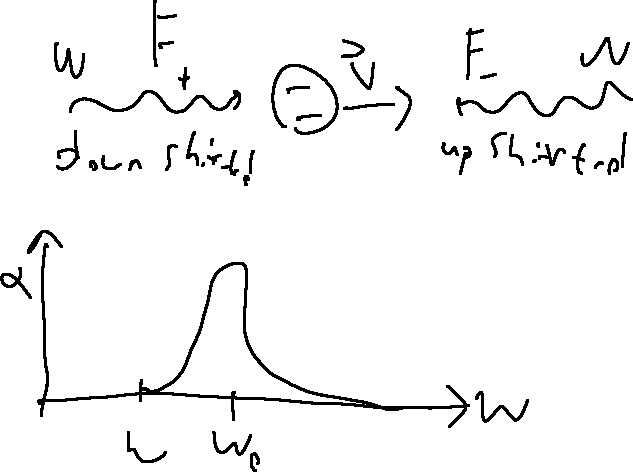
\includegraphics[width=10cm]{images/11-26-6.png}
	\caption*{Doppler cooling}
\end{figure*}
For doppler cooling we have two optical fields incident on an atom in opposite directions. By choosing $\omega$ less than $\omega_0$ we cause the force applied by the laser in the opposite direction of the motion to be greater than the one in the direction of motion.
This leads to a cooling/fricitional force/cooling force. We will eventually show $F\propto v$.
